\chapter{The blood microbiome}

\section{Importance of the microbiome}

In an adult human, the bacteria within the colon alone outnumbers host cell numbers by up to two orders of magnitude, resulting in least 100-fold more bacterial genes relative to human \cite{Brenchley:2012bm}. The importance of the microbiome has become evident through studies of germ-free animals: these are more susceptible to infections and have reduced vascularity, digestive enzyme activity, muscle wall thickness. Numerous studies have implicated an altered balance in the composition of the microbiota (dysbiosis) in many diseases, such as obesity, celiac disease, type 2 diabetes, atopic eczema, asthma, inflammatory bowel disease (IBD), and chronic diarrhea  \cite{Brenchley:2012bm}.

\section{Linking blood and body sites}

The Human Microbiome Project defined the compositional range of the microbiome within healthy individuals \cite{Consortium:2012bb}. Since this pioneering work, the microbiome in different physiological contexts has become intensely studied. Pregnancy is one important example, as preterm birth is a leading cause of neonatal mortality and can be driven by intrauterine infections. Until recently, it was thought that intrauterine infections originated in the lower genital tract and microbiota ascended into the otherwise sterile womb environment \cite{Prince:2014gx}. Recent studies have shown that the microbiome changes during pregnancy according to hormonal and physical fluctuations \cite{Koren:2012ji} and, in addition, the human placenta is not sterile. Rather, the placenta harbors a unique microbiome with taxonomic composition similar to the oral cavity. As a result of this work, evidence suggests that the placenta may be seeded by microbes traveling through blood from other body sites and changes in the placenta microbiome may influence adverse pregnancy outcomes \cite{Aagaard:2014vk}.

If blood serves as a transmission medium for micro-organisms over the course of pregnancy, then it may serve as a useful diagnostic indicator and may be useful to measure. Recent work has shown that micro-organism derived cell-free DNA fragments can be purified from blood and counted via next-generation sequencing (NGS) \cite{DeVlaminck:2013hl}. Though much of this material is likely the detritus of dead and apoptosed cells \cite{Quake:2012iy}, the sources for this material are unclear. With this in mind, we shotgun sequenced cell-free DNA from fifty eight plasma samples within a cohort of fourteen women enrolled in a clinical study at Stanford hospital. For each sample, we isolated and analyzed micro-organism derived cell-free DNA. For each blood sample, we performed temporally matched 16s sequencing from four body sites (Saliva, Vagina, Gut, and Gum) on the same patient.

We first performed descriptive analysis of the data by comparing the taxonomic composition of blood relative to the sampled body sites at genus-level resolution. We discretized mean fractional abundance data for blood and all sampled body sites, resulting in a binary value for each genus. We then compared the genus detected in blood to genus detected in body sites. $58$\% of the genus detected in the body sites were also found in blood, while only $15$\% of the genus detected in blood were detected in any body site. This suggested that micro-organism derived material in blood originates from more than just the sampled sources (Figure ~\ref{fig:Fig12}).

\begin{figure*}
\center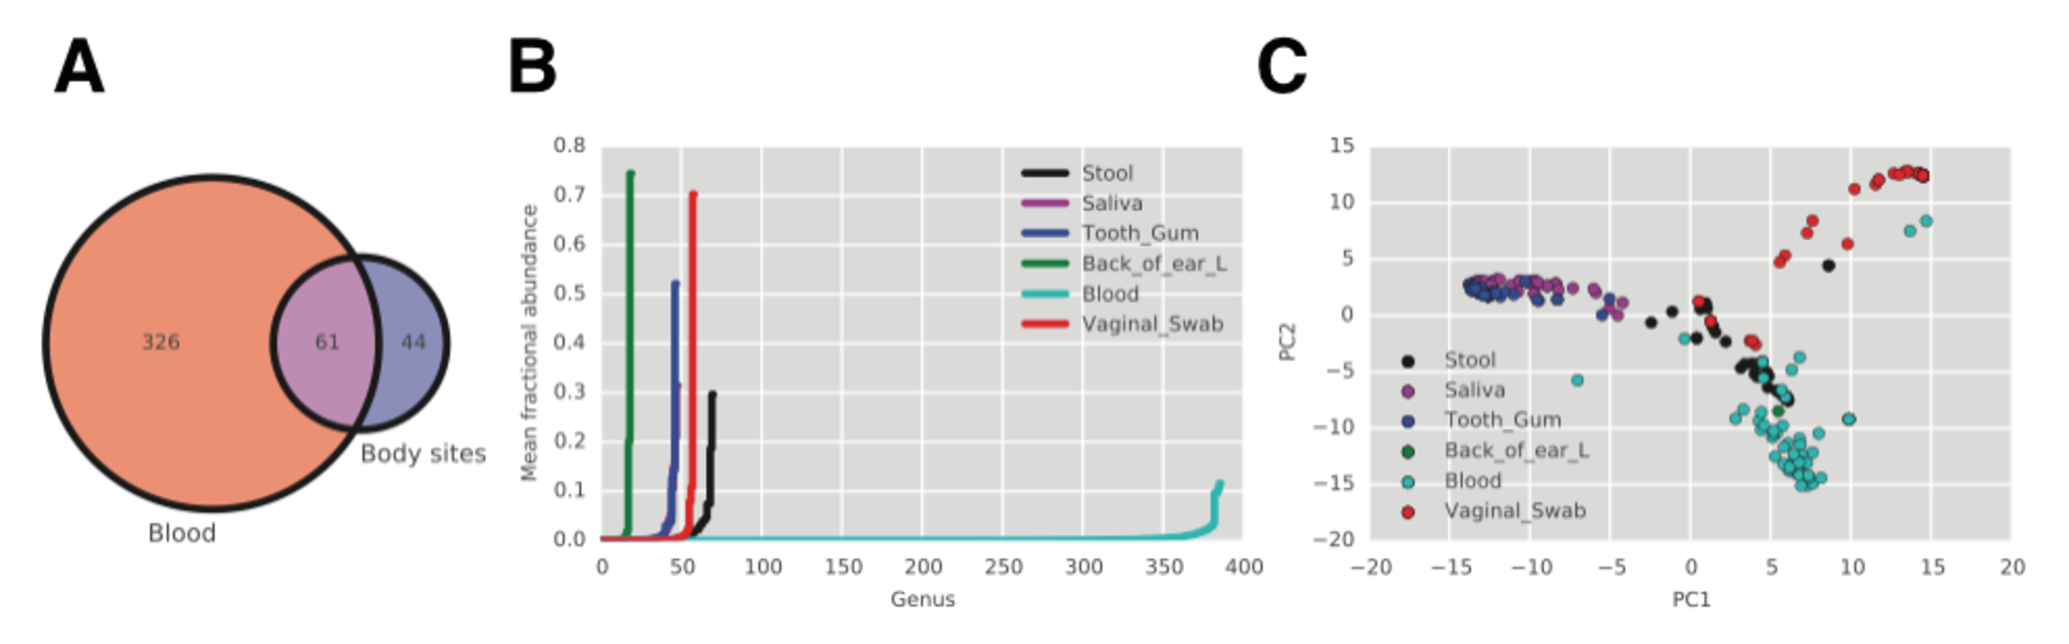
\includegraphics[width=150mm,scale=0.5]{Figures/Fig12}
\caption{Composition of the blood microbiome}
\label{fig:Fig12}
\end{figure*}

We then evaluate the distribution of mean fractional abundances for each site. The 16s sampled body sites showed strong enrichment in particular genus that are known to be well-adapted to each biological niche \cite{Consortium:2012bb}. Blood is quite different: the number of genus detected is $\approx 8$-fold greater than the body sites, with a mean fraction abundance $\approx 10$-fold lower than the body sites. We transformed the data using PCA in order to determine the genus that most strongly drive the measured variation in blood as well as the sampled tissues (Figure ~\ref{fig:Fig12}). PCA indicated that blood samples generally cluster together in taxonomic space and occupy a distinct compositional niche relative to the sampled body sites. We examined genus that strongly contribute to the principal components in order to understand what distinguishes blood from the body sites: as expected, genus - notably, Acidovorax and Cupriavidus - that drive the variation are found at high fractional abundance in the blood samples, but are nearly absent from the sampled body sites. 

We next investigated whether blood samples each body site. We reasoned that body-site specific micro-organisms provide a reasonable indicator for this. We compute specificity by discretizing the genus found in each body site and comparing the profile of each body site to all genus found in all other sites (Figure ~\ref{fig:Fig13}). For this analysis, we used our sampled body site data as well as the metagenomic community profiles made available by the Human Microbiome Project \cite{Consortium:2012bb}, which contains 35 billion reads taken from 690 samples from 300 US subjects across 15 body site. 

In both cases, we computed a list of body-site specific genus, which were only detected in single body sites for all samples collected. We then asked whether these genus were ever detected in blood: we detected $57$\% and $45$\% of the site-specific genus in blood determined via HMP metagenomic community profiles and the 16s data collected for this study, respectively. We then asked whether the site-specific absent from blood were found at lower abundance in the sampled tissues. We found no significant difference between the abundance between site specific genus detected and un-detected in blood, which argues against the possibility that under-sampling is likely to explain failure to detect all site-specific genus. 

\begin{figure*}
\center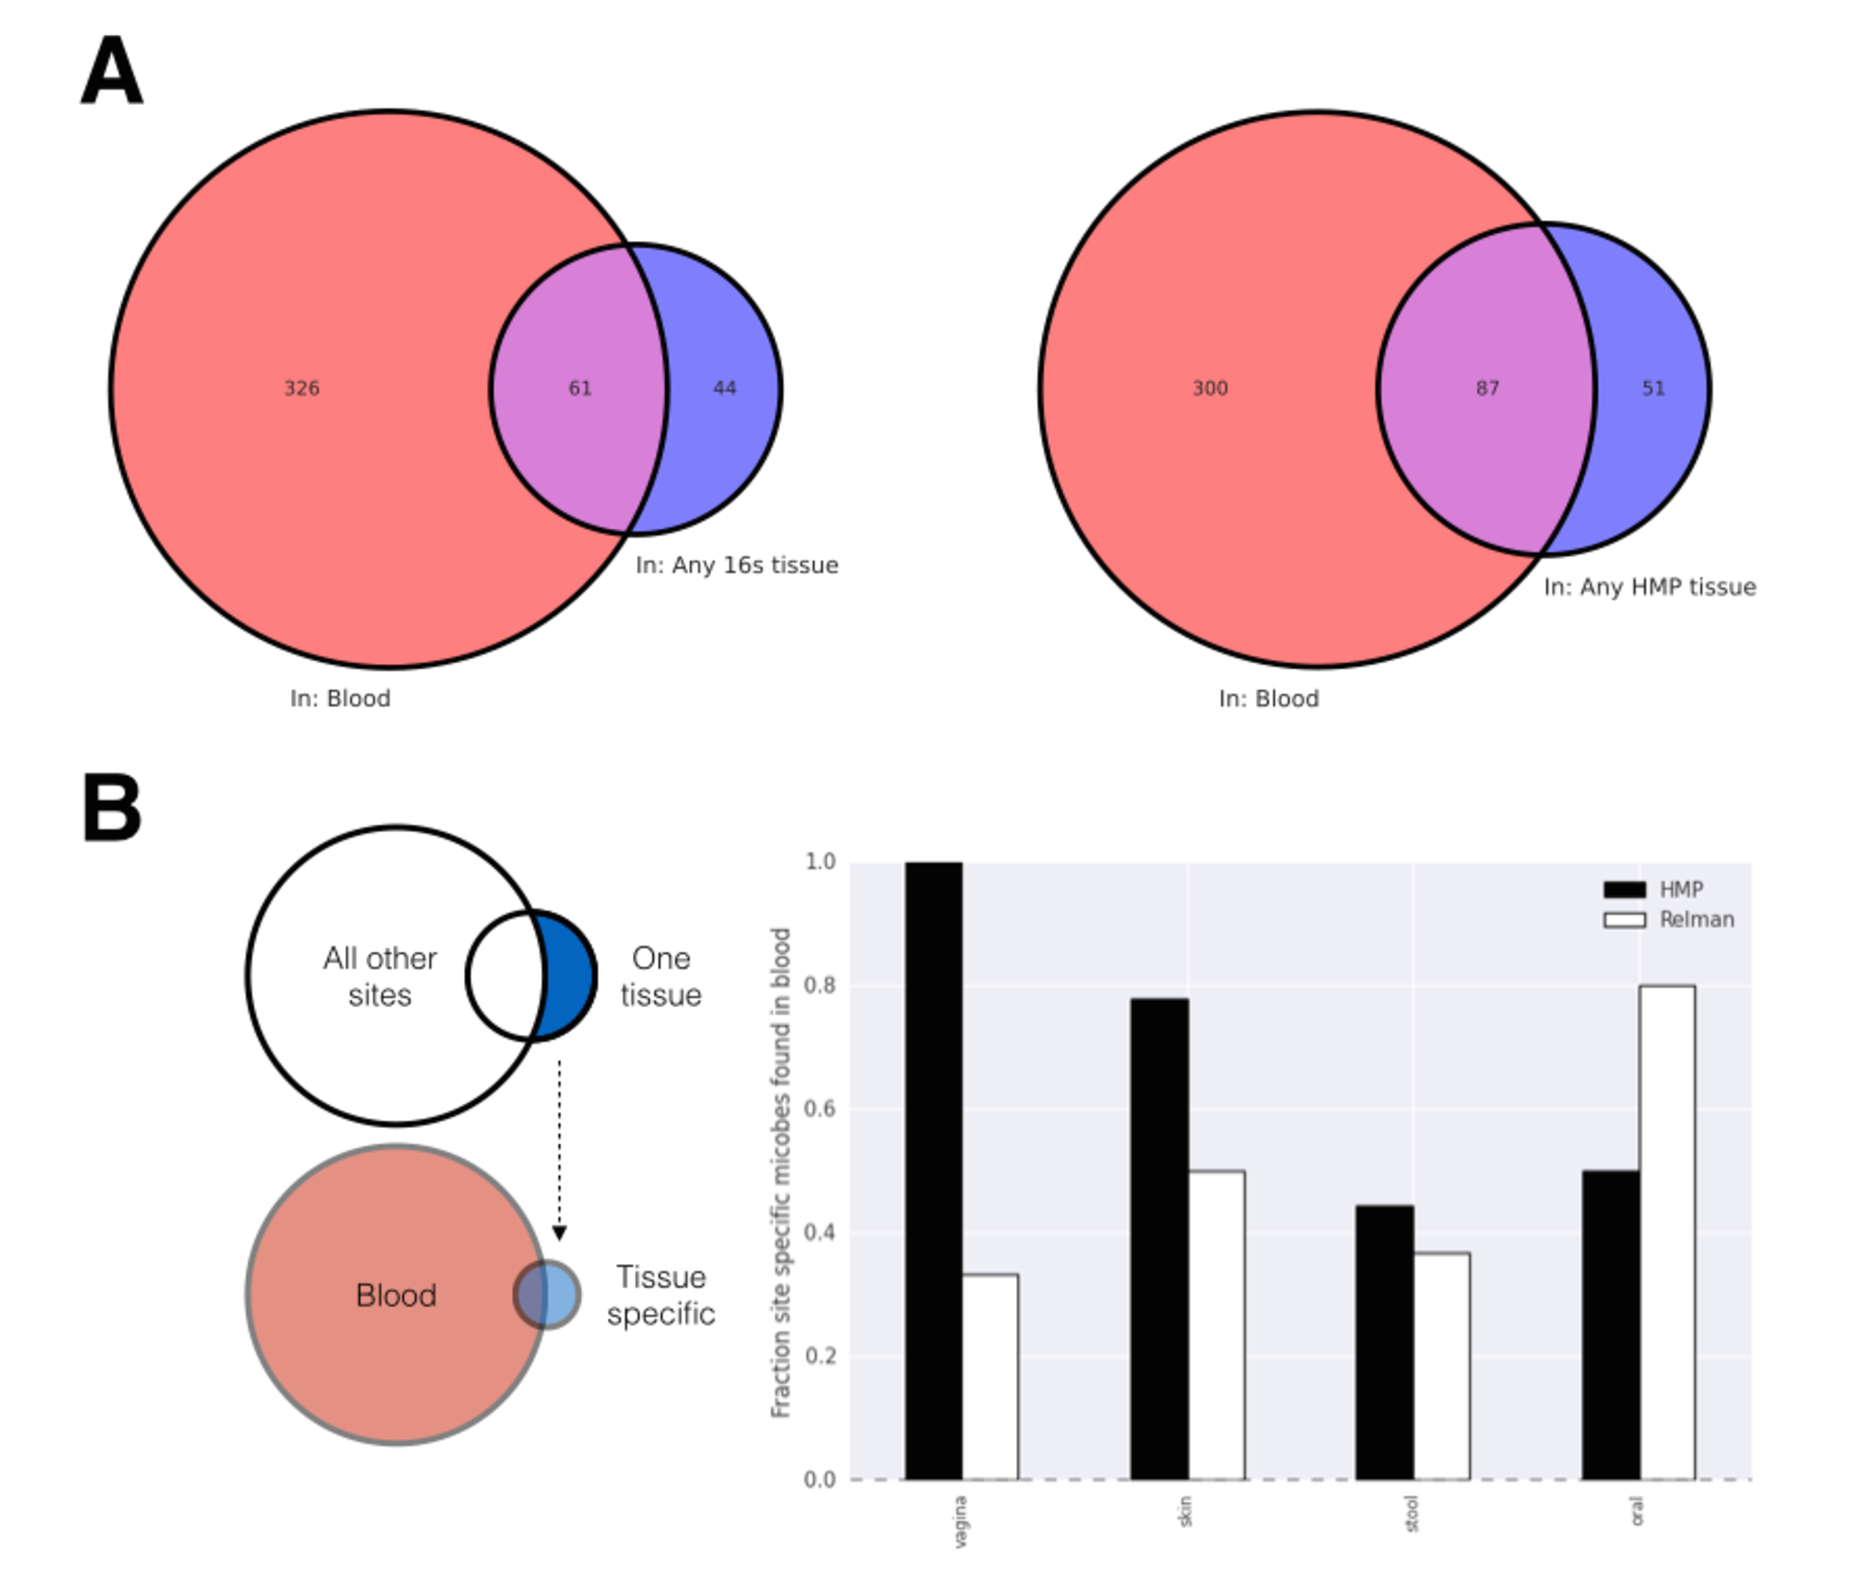
\includegraphics[width=150mm,scale=0.5]{Figures/Fig13}
\caption{Detection of body site specific bacteria in blood.}
\label{fig:Fig13}
\end{figure*}

From this analysis, we obtained an assignment of body site specificity for each genus detected in our data. Any each genus was either assigned to a specific body site or deemed mixed source, meaning that it was detected in more than one body site. We partitioned the genus detected in blood using this assignment in order to gain insight into their origin. This analysis indicated that blood is composed primarily of two types: genus derived from mixed sources, which cannot be traced to any specific tissue, and genus that are specific to blood only (Figure ~\ref{fig:Fig14}).

\begin{figure*}
\center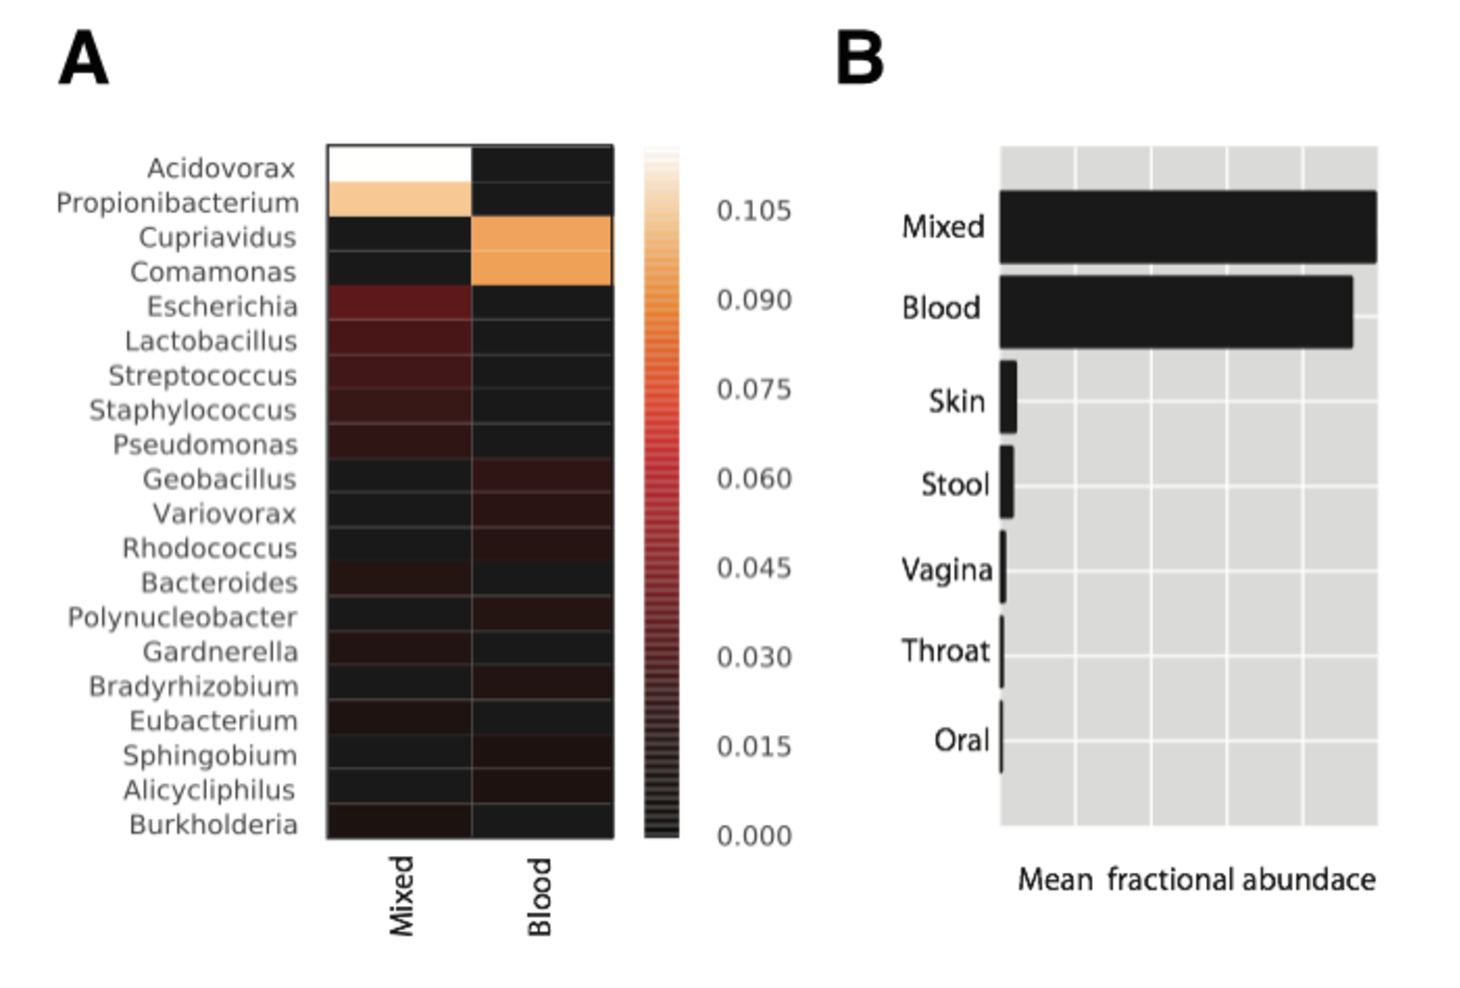
\includegraphics[width=120mm,scale=0.5]{Figures/Fig14}
\caption{Likely sources for most abundant bacteria detected in blood.}
\label{fig:Fig14}
\end{figure*}

\section{Coupling between blood and body sites}

We then asked if a physical relationship between genus found in blood and  body sites can be established. Specifically, we examine whether the fractional abundance of genus at any body site is linked to detection in blood. In order to do this, we discretized the blood data for each sample. For each genus, we then evaluated the fractional abundance of that genus for all matched body site samples. We compared the distribution of abundances at each body site based upon whether the genus was found in blood, expecting a difference in distribution if a body site was obviously coupled to blood (e.g., an elevation in abundance at a tissue when the genus was found in blood). However, found no signifiant difference between the body site fractional abundance with respect to detection in blood. 

We further examined whether the composition of genus detected in blood can be modeled as a function of the sampled sites. We chose a linear model, meaning that each blood sample was modeled as a linear combination of the genus at temporally matched body sites. We used a quadratic programming package to determine the mixing coefficients that minimize the squared error between the model and the blood measurement, subject to intuitive constraints (e.g., the coefficients must be greater than zero). After confirming the solver works correctly by recapitulating the correct mixing coefficients on simulated data, we applied it to all samples. 

\begin{figure*}
\center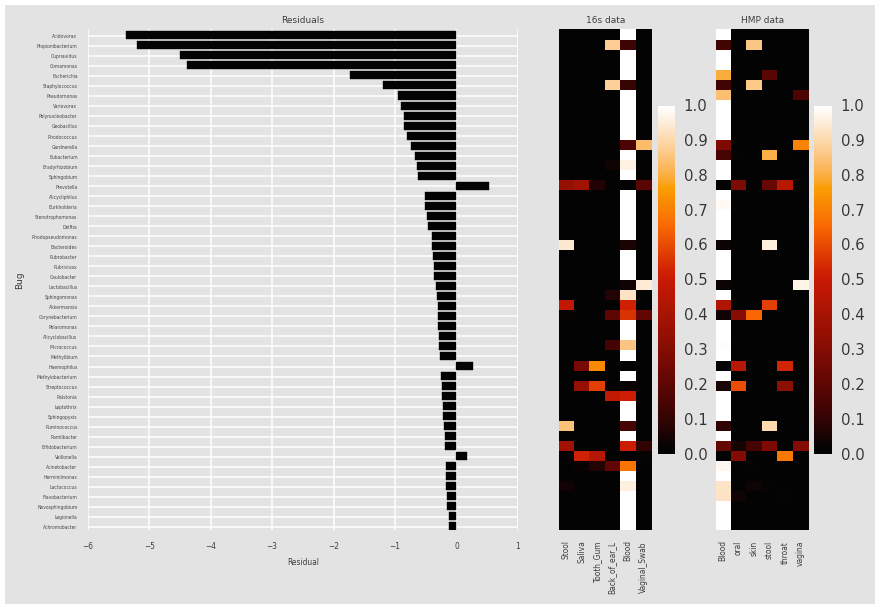
\includegraphics[width=150mm,scale=0.5]{Figures/Fig14_2}
\caption{Residuals from linear regression.}
\label{fig:Fig14_2}
\end{figure*}

We found that the model performed poorly, using coefficient of determination ($r^2$) between the model guess and actual blood data as a measure of fit. However, examination of the the residuals was informative: intuitively, we found that the model fails because many highly abundant genus detected in blood are not found in the sampled body sites. In order words, the sampled sources are insufficient to describe the composition of blood, as blood apparently samples from additional tissues or serves as an environment that amplifies specific genus non-linearly.

\section{Summary}

The abundance distribution of genus in blood is different than sampled body sites. Sampled body sites are dominated by few genus at high abundance with a relatively short tail of low-abudnance genus. This reflects the fact that some genus are well-adapted to each body site niche. Blood contains many more genus, but at far lower fractional abundance and a long tail of genus found at trace abundance. Blood may serve as a common sink into which all tissues contribute dead cells, resulting in a passive environment of mixed DNA fragments that we sampled. We also found that most abundant genus in blood are essentially absent from sampled body sites. This suggests that either that blood can samples from more sources (e.g., internal tissues) or that blood may be a niche for a certain, narrow sub-set of genus. 

Analysis of site-specific genus provides evidence that blood samples each body site, as around half of site specific genus are found in blood when analyzed at both genus and species-level resolution using both our body site data as well as the HMP data. However, we did not find clear evidence of coupling between body sites and blood: there is not apparent difference in genus abundance at any body site based upon whether that genus is detected in blood in a temporally matched sample. This is not surprising: the blood is under-sampled, meaning that few of the present microorgaism-dervied fragments are actually sequenced in our data, and blood is a complex mixture represent many tissue sources. The latter point also frustrated efforts to model blood as a function of the sampled sites: blood data contains genus that were not detected in any of the sampled tissues. 
